% !TEX root = _yoko.tex

% ==========================================
% プロジェクト予稿（1P）の本文
% ==========================================

\section{はじめに}
% 音は，視覚に依存しない情報伝達手段として幅広く利用されている．しかし，物語という複数のイベントの連続で構成される作品形式において，音によって意図された出来事や感情が，どのように聴者に知覚されるのかについては，十分に検討されていない．そこで本研究では，音による情報伝達を物語表現に適用する試みとして，音のみを用いた物語作品を制作し，制作者の意図した出来事や感情が，聴者にどのように知覚されるのかを検討することを目的とする．
音は視覚に依存しない情報伝達手段として，環境音や警告音，音楽表現など，
さまざまな文脈で利用されてきた．
一方で，複数の出来事や感情の変化によって構成される「物語」という形式において，
音のみを用いて制作者の意図した状況や意味が，
どのように聴取者に知覚されるのかについては，
十分に整理されていない．


本研究では，音による意味伝達を物語表現に応用する試みとして，
音のみを用いた物語作品を制作し，
その構成および音響設計を整理するとともに，
実演を通じて，聴取時の知覚について確認することを目的とする．

\section{音による意味伝達と物語表現}
本研究の背景として，
（１）音が出来事や環境を知覚させる手がかりとなること\cite{gaver_what_1993}，
（２）音による情報伝達が設計の問題として捉えられてきたこと（ソニフィケーション研究\cite{hermann_taxonomy_2008,kramer_sonification_nodate}）を踏まえている．
これらの先行研究では，音による意味伝達は可能である一方で，
その有効性は文脈や配置に強く依存し，事前に一意の正解が定まるものではないことが指摘されている．
本研究は，こうした理論的背景を踏まえ，
音のみを用いた物語作品の制作を通じて，
音響設計と物語理解との関係を整理する試みとして位置づけられる．

\ModifyHeading{section}{lines=2}
\section{音のみを用いた物語作品の制作}
\ModifyHeading{section}{lines=1}

%本研究では，事故により飛行不能となったハチドリを主人公とし，地上の動物との関わりを経て再び飛行に至る過程を描いた，音のみで構成される物語作品『日暮どきこそ耳を澄まして：「Echo」～音だけの動物物語～』を制作した．本作品では，サンプリングした音声素材を主にMIDIデータとして扱い，ピッチやタイミングの演奏情報の制御を通じて，物理的な動きや登場キャラクターの感情表現をおこなった．
%さらに，第三者を対象として本作品を実演し，実際の聴取における知覚を確認して結果，音のみで構成された物語表現においては、制作者の意図した出来事や感情が必ずしも十分に伝達されないことが明らかとなった。

本研究では，アクシデントにより飛行不能となったハチドリを主人公とし，地上の動物との関わりを経て再び飛行に至るまでの過程を描いた，音のみで構成される物語作品\textbf{『日暮どきこそ耳を澄まして：「Echo」～音だけの動物物語～』}を制作した．

本作品では，登場キャラクターを動物に限定し，背景音や発声音，動作音といった音響イベントの連なりによって，場面の変化や物語の進行を表現している．音素材は主にサンプリングによって収集し，MIDI音源として扱うことで，ピッチやタイミングといった演奏情報を制御し，動きや感情の変化を音響的に表現した．
また，作品全体を複数の場面に分割し，各場面において背景音と音響イベントの対応関係を整理することで，物語構造と音響設計の関係を明示した．

\section{制作環境}
本作品の制作にあたっては，音響編集ソフトウェアおよびMIDIシーケンス環境を用い，
音素材の整理，配置，および再構成を反復的に行った．
特定の設計理論に基づいて一度で完成させるのではなく，
音響イベントの組み合わせや時間的配置を試行錯誤しながら調整することで，
聴取者にとって出来事や感情の変化がどのように知覚されるかを確認しつつ制作を進めた．
このような制作過程を通じて，音による意味伝達が
文脈や配置に大きく依存することを実感的に捉えることを目指した．

特に，背景音や環境音を物語進行の手がかりとして用いることで，
明示的な説明を伴わずに場面の転換や状況の変化を示すことを意識した．

\section{実演と考察}
\begin{figure}[t]
    \centering
    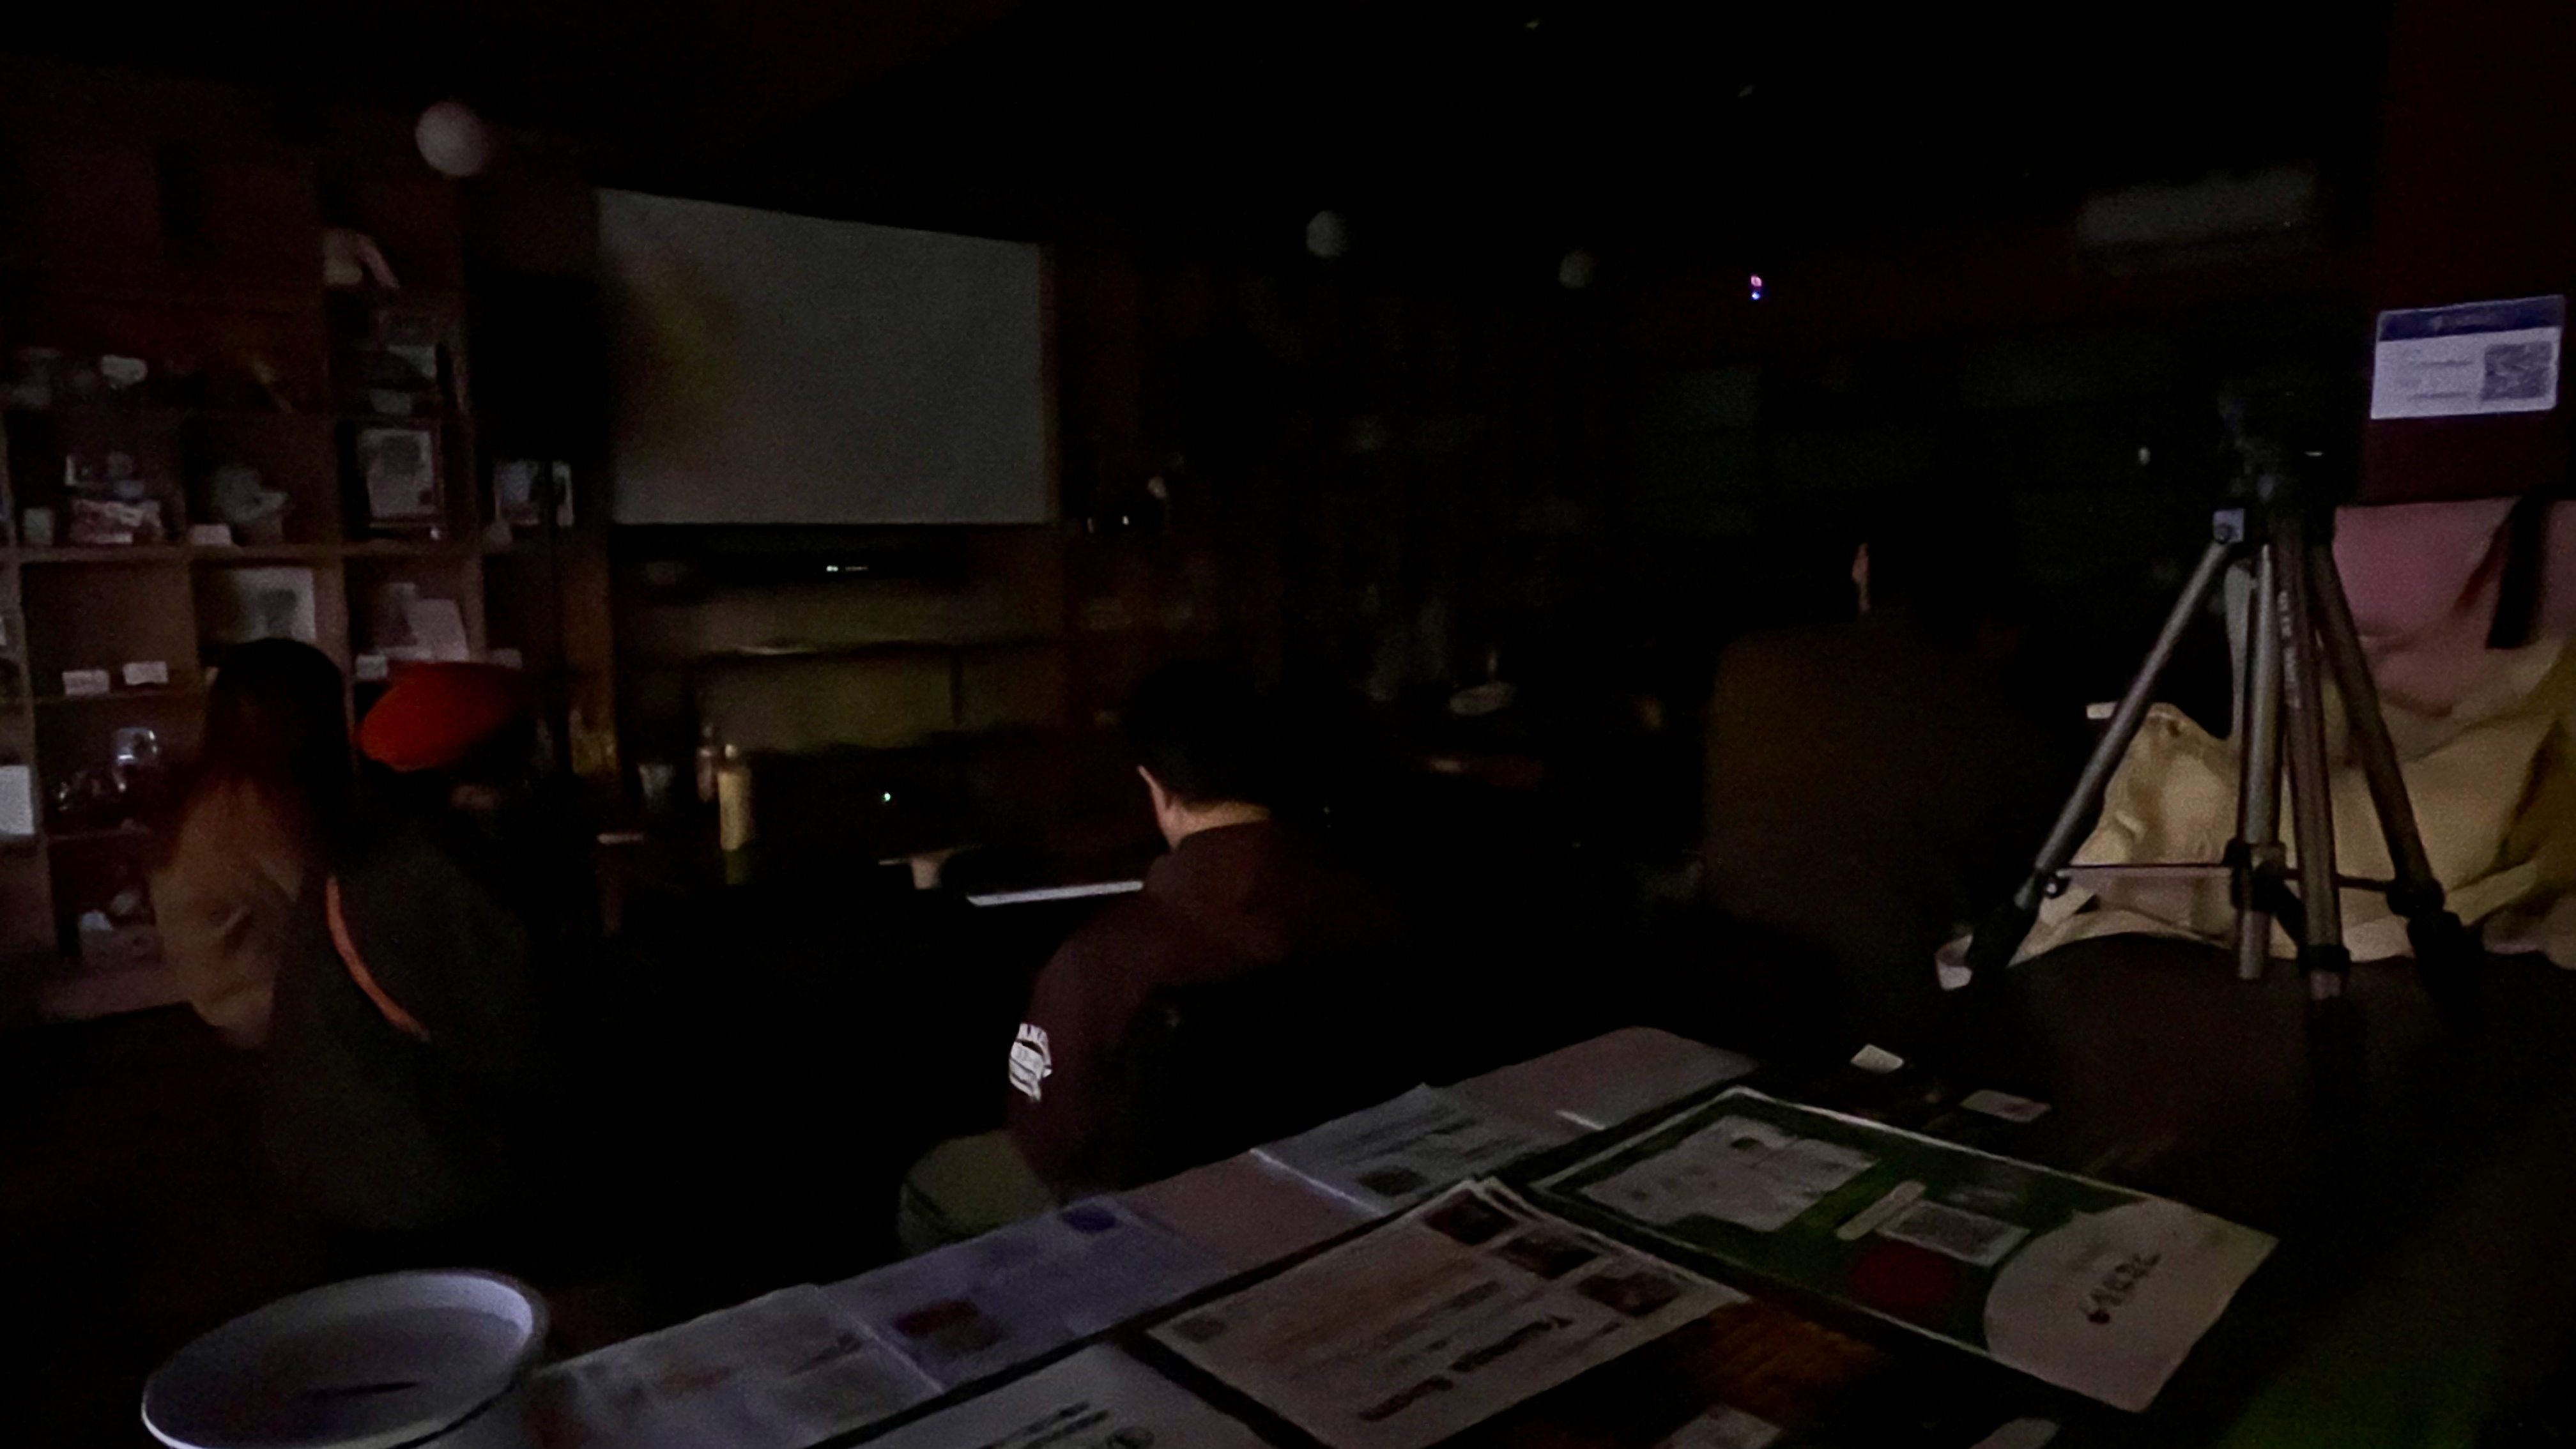
\includegraphics[width=\hsize]{1220oto.png}
    \caption{作品実演の様子}\label{fig:1220oto}
\end{figure}

制作した作品について第三者を対象とした実演を行い，聴取後の反応や感想を通じて，物語内容の知覚について確認を行った．その結果，音のみで構成された物語表現においては，一部の出来事や感情について制作者の意図と聴取者の理解が一致する一方で，場面の転換や因果関係については，必ずしも十分に伝達されない場合があることが示唆された．
これらの結果から，音による物語表現においては，音響イベントの配置や変化の明確さが，出来事や感情の理解に大きく影響することが示された．

このことは，音のみを用いた物語表現において，
音響イベントを単独で配置するだけでなく，
それらの時間的な連なりや変化の方向性を
どのように構成するかが重要であることを示している．
本作品の制作を通じて，
物語理解は特定の音素材そのものよりも，
背景音と出来事音との関係性や，
それらの推移の中で知覚される文脈に
強く依存することが確認された．

本研究は，音のみを用いた物語表現の構成と音響設計について整理し，
その可能性と課題を示す一事例として位置づけられる．